\subsubsection{GPUs in Computers}

Two main computer GPU setups are prominent today: \textit{integrated} graphical processing units (iGPU), and \textit{discrete} graphical processing units (dGPU).
iGPUs are GPUs integrated onto the same die as a computer's CPU, where the two share the same physical \textit{Random Access Memory} (RAM) unit.
dGPUs are dedicated GPU devices that are physically distinct from the host computer's CPU and RAM, and have their own physical RAM.
dGPUs are significantly more powerful in terms of compute throughput when compared to iGPUs.
However, having their own physical RAM introduces an overhead;
Memory buffers with input data have to be copied to the dGPU's RAM before processing, and results have to be copied back from the dGPU's RAM to the host RAM.

\begin{figure}[h!]\label{figure:igpu-and-dgpu-system}
\begin{center}
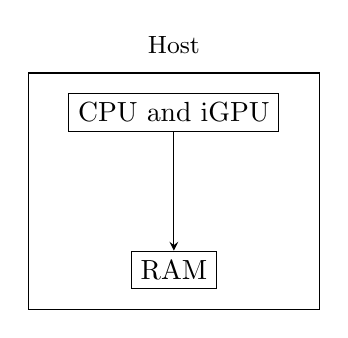
\begin{tikzpicture}
  % draw die
  \node at(0,2)[rectangle,draw](cpu){CPU and iGPU};
  % draw RAM
  \node at(0,0)[rectangle,draw](ram){RAM};
  % draw "Host" text
  \node at(0,2.85){\small Host};
  % draw host computer
  \node at(0,1)[rectangle,draw,minimum width=3.7cm,minimum height=3cm](dualhost){};
  % draw arrow from die to RAM
  \draw [-stealth](cpu) -- (ram);
\end{tikzpicture}
\hspace{8em}
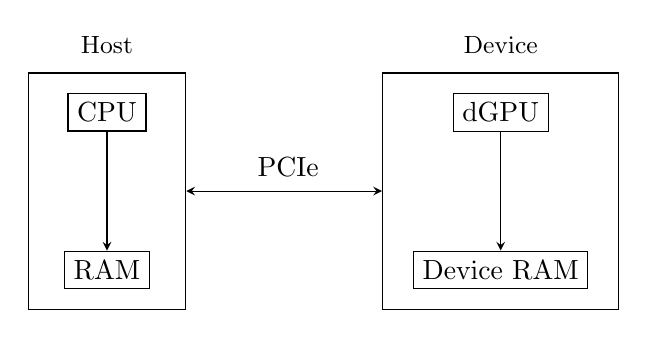
\begin{tikzpicture}
  % draw CPU die
  \node at(0,2)[rectangle,draw](cpu){CPU};
  % draw host RAM
  \node at(0,0)[rectangle,draw](cpuram){RAM};
  % draw dGPU die
  \node at(5,2)[rectangle,draw](gpu){dGPU};
  % draw host RAM
  \node at(5,0)[rectangle,draw](gpuram){Device RAM};
  % draw host computer
  \node at(0,1)[rectangle,draw,minimum width=2cm,minimum height=3cm](host){};
  % draw device
  \node at(5,1)[rectangle,draw,minimum width=3cm,minimum height=3cm](device){};
  % draw arrow from CPU die to host RAM
  \draw [-stealth](cpu) -- (cpuram);
  % draw arrow from dGPU die to device RAM
  \draw [-stealth](gpu) -- (gpuram);
  % draw arrow to and from host and device
  \draw [stealth-stealth](host) -- (device);
  % draw "PCIe" text
  \node at(2.3,1.3){\smaller PCIe};
  % draw "Host" text
  \node at(0,2.85){\small Host};
  % draw "Device" text
  \node at(5,2.85){\small Device};
\end{tikzpicture}
\caption{\textbf{Left}: A computer setup with a CPU and an iGPU sharing the same die and the same physical RAM. \textbf{Right}: A computer setup where a dGPU is connected over PCIe and the dGPU has its own physical RAM, adding the overhead of copying data both to and from the host computer when utilizing the GPU.}
\end{center}
\end{figure}

For the work presented in this thesis, only dGPUs were utilized. 
Therefore, the term GPU will from here on out be referring to a dGPU and not an iGPU.
This means that all GPU implementations discussed in this thesis will include copying memory back and fourth from the \textit{host} (CPU) RAM and the \textit{device} (GPU) RAM.
It is also possible for a single computer to have several connected GPUs, allowing for further parallelization of both memory transfers and compute, however this was not utilized in this thesis' work.
